\documentclass[conference]{IEEEtran}
\IEEEoverridecommandlockouts
% The preceding line is only needed to identify funding in the first footnote. If that is unneeded, please comment it out.
\usepackage{cite}
\usepackage{amsmath,amssymb,amsfonts}
\usepackage{algorithmic}
\usepackage{graphicx}
\usepackage{textcomp}
\usepackage{xcolor}
\usepackage{booktabs}
\usepackage{microtype}
\usepackage{url}
\usepackage{stfloats}
\usepackage{placeins}

% Float parameters to prevent tables and figures from dumping after references
\setcounter{topnumber}{5}
\setcounter{bottomnumber}{5}
\setcounter{totalnumber}{10}
\setcounter{dbltopnumber}{5}
\renewcommand{\topfraction}{0.95}
\renewcommand{\bottomfraction}{0.95}
\renewcommand{\textfraction}{0.05}
\renewcommand{\dbltopfraction}{0.95}
\renewcommand{\dblfloatpagefraction}{0.8}

\def\BibTeX{{\rm B\kern-.05em{\sc i\kern-.025em b}\kern-.08em
    T\kern-.1667em\lower.7ex\hbox{E}\kern-.125emX}}

\begin{document}

\title{AI-Based Rooftop Solar Potential Assessment Using Satellite Imagery}

\author{
\begin{tabular}[t]{c@{\hspace{2.2em}}c@{\hspace{2.2em}}c}
Aryan Mishra & Sarang Palsutkar & Abhinav Verma \\
\textit{School of Computing Sci. \& Eng.} & \textit{School of Computing Sci. \& Eng.} & \textit{School of Computing Sci. \& Eng.} \\
\textit{VIT Bhopal University} & \textit{VIT Bhopal University} & \textit{VIT Bhopal University} \\
Bhopal, India & Bhopal, India & Bhopal, India \\
{\footnotesize aryan.23bce11833@vitbhopal.ac.in} & {\footnotesize sarang.23bce11382@vitbhopal.ac.in} & {\footnotesize abhinav.23bce11377@vitbhopal.ac.in} \\[2.2ex]
\multicolumn{3}{c}{%
\begin{tabular}[t]{c@{\hspace{4.5em}}c}
Pratik Rajendra Kolhe & Sanvi Tikariha \\
\textit{School of Computing Sci. \& Eng.} & \textit{School of Computing Sci. \& Eng.} \\
\textit{VIT Bhopal University} & \textit{VIT Bhopal University} \\
Bhopal, India & Bhopal, India \\
{\footnotesize pratik.23bce11399@vitbhopal.ac.in} & {\footnotesize sanvi.23bce11603@vitbhopal.ac.in}
\end{tabular}%
}
\end{tabular}
}

\maketitle

\begin{abstract}
Automated mapping of distributed rooftop solar photovoltaic (PV) installations from overhead satellite and aerial imagery is essential for modern distribution grid operations, hosting capacity auditing, and urban renewable energy planning. However, models trained on clean single-source aerial surveys frequently collapse when deployed across multi-resolution satellite platforms due to zoom scale shifts, atmospheric degradation, and false positives triggered by dark shingles, skylights, and asphalt surfaces. In this work, we conduct a progressive investigation bridging exploratory baseline architectures and cross-literature state-of-the-art benchmarks. First, we benchmark five distinct baseline paradigms (Mask R-CNN, U-Net, DeepLabV3+, SegFormer, and YOLOv8m-seg) on high-resolution aerial orthomosaics, identifying Vision Transformers as having superior capacity for global structural modeling. To overcome single-domain failure modes, we develop a Multi-Scale Domain-Invariant SegFormer (MiT-B2) trained on a massive multi-source corpus of 2,957 tiles integrating Google Earth Engine satellite imagery, multi-roof UAV surveys, and aerial orthomosaics with explicit hard-negative mining and multi-scale test-time augmentation (TTA). We then benchmark our model directly against official open-source weights from published literature (Fraunhofer ISE DeepLabV3+, UPM UNet++ and YOLOv8-seg, and Microsoft Global Renewables Watch U-Net) on a single frozen test set of 400 images from the BDAPPV benchmark (\textit{Nature Scientific Data}, 2023). Our proposed model achieves state-of-the-art performance, recording 81.43\% mIoU, 0.8977 F1-score, and 99.79\% pixel accuracy, outperforming all published literature baselines while operating at 24.3 FPS on an NVIDIA Tesla T4 GPU.
\end{abstract}

\begin{IEEEkeywords}
Solar photovoltaic detection, semantic segmentation, Vision Transformers, remote sensing, cross-literature benchmark, SegFormer, deep learning, Geospatial AI.
\end{IEEEkeywords}

\section{Introduction}
Decentralized rooftop solar photovoltaic (PV) generation has emerged as a cornerstone of urban decarbonization and clean energy transitions \cite{b_geoai}. In contrast to centralized utility-scale solar farms, residential and commercial rooftop arrays are spatially fragmented, architecturally diverse, and often unmetered in official utility cadastres. Distribution system operators (DSOs) and municipal energy authorities require automated, accurate spatial inventories of existing PV installations to maintain voltage stability, schedule substation hosting capacity, and simulate feeder peak load reversibility \cite{b_bdappv}.

While deep learning architectures applied to remote sensing imagery offer an attractive alternative to manual ground inspections \cite{b_jiao}, deploying models in real-world geospatial applications presents severe domain-shift challenges:
\begin{enumerate}
    \item \textit{Scale Shift Across Zoom Levels}: Satellite imagery acquired from mapping platforms (e.g., Google Earth Engine) fluctuates across zoom levels 18, 19, and 20, altering solar panel pixel dimensions by over 400\% for identical physical installations.
    \item \textit{The Hard-Negative Trap}: Unoccupied asphalt shingles, dark roof membranes, skylights, air conditioning ducts, and road surfaces exhibit spectral signatures nearly identical to monocrystalline silicon modules. Models trained exclusively on solar-positive chips suffer from acute false-positive inflation when deployed over suburban extents.
    \item \textit{Sensor Heterogeneity and Atmospheric Haze}: Variances in solar azimuth, ground sampling distance (GSD), and lossy JPEG compression artifacts degrade boundary crispness.
\end{enumerate}

To resolve these challenges, this paper presents a three-stage research progression:
\begin{itemize}
    \item \textbf{Stage 1: Exploratory Baseline Benchmark}: A comprehensive comparison of five leading deep learning paradigms (Mask R-CNN, U-Net, DeepLabV3+, SegFormer, and YOLOv8m-seg) trained on sub-meter aerial orthomosaics, isolating Vision Transformers as the most structurally robust framework.
    \item \textbf{Stage 2: Multi-Scale SegFormer Scaling}: Expanding the training corpus to 2,957 multi-source tiles across Google Earth, UAV, and aerial platforms with scale-invariant multi-scale training ($0.4\times$ to $1.6\times$) and explicit hard-negative mining.
    \item \textbf{Stage 3: Cross-Literature SOTA Benchmark}: An apples-to-apples empirical evaluation comparing our proposed Multi-Scale SegFormer directly against published pretrained models from Fraunhofer ISE, UPM Madrid, and Microsoft Nature on a single frozen test set from the BDAPPV benchmark \cite{b_bdappv}.
\end{itemize}

\section{Related Work}
Existing literature on automated overhead solar photovoltaic mapping falls into three dominant architectural paradigms:

\subsection{Two-Stage and Single-Stage Detectors}
Two-stage instance segmentation frameworks, such as Mask R-CNN \cite{b_maskrcnn}, isolate candidate region proposals via a Region Proposal Network (RPN) before performing RoIAlign feature extraction and mask prediction. While two-stage models provide strong boundary localization on isolated roofs, their computational latency ($>35\text{ ms/chip}$) limits metropolitan scaling. Single-stage anchor-free instance segmenters, including YOLOv8-seg \cite{b_yolo}, combine prototype masks with predicted coefficient vectors to maximize inference throughput ($>90\text{ FPS}$), though frequently exhibiting boundary over-smoothing on compact residential arrays.

\subsection{Encoder-Decoder Convolutional Networks}
Symmetric encoder-decoder networks transfer high-resolution spatial details across contracting and expanding paths via skip connections. The classical U-Net \cite{b_unet} and its nested variants (UNet++) \cite{b_moreno} preserve fine pixel coordinates of module edges. Multi-scale context aggregation models, such as DeepLabV3+ \cite{b_deeplab}, integrate Atrous Spatial Pyramid Pooling (ASPP) to expand receptive fields without loss of spatial resolution, as demonstrated by Kleebauer et al. \cite{b_kleebauer} for multi-resolution solar mapping.

\subsection{Vision Transformers and Planetary Foundation Models}
Recent advances in hierarchical Vision Transformers, notably SegFormer \cite{b_segformer}, replace traditional convolutions with spatial-reduction self-attention mechanisms. By capturing global spatial dependencies without positional embedding interpolation bottlenecks, transformer backbones achieve superior resilience to local textural confounding. Planetary-scale foundation efforts, such as Microsoft's Global Renewables Watch (GRW) \cite{b_grw}, deployed U-Net models on Sentinel-2 imagery; however, their coarse resolution targets utility-scale solar farms, failing to resolve decentralized residential rooftop systems.

\section{Exploratory Baseline Study}
To establish baseline capabilities, our research team implemented and benchmarked five distinct deep learning paradigms under identical experimental constraints.

\subsection{Baseline Dataset and Experimental Setup}
The initial exploratory benchmark utilized high-resolution ($0.15\text{ m/pixel}$) aerial orthophotography covering Davis, California:
\begin{itemize}
    \item \textit{Spatial Tiling}: Orthomosaics were chipped into $W_c = 512, H_c = 512$ pixel tiles with a spatial stride of $S = 256$ pixels (50\% spatial overlap) to avoid boundary truncation.
    \item \textit{Vector Ground Truth}: Cadastral GeoJSON layers comprising $1,420$ verified rooftop solar panel boundaries were rasterized to binary ground-truth masks.
    \item \textit{Training Protocol}: All five models were trained on an NVIDIA Tesla T4 GPU using cosine learning rate scheduling and early stopping with patience $p = 7$.
\end{itemize}

\begin{figure}[t]
\centering
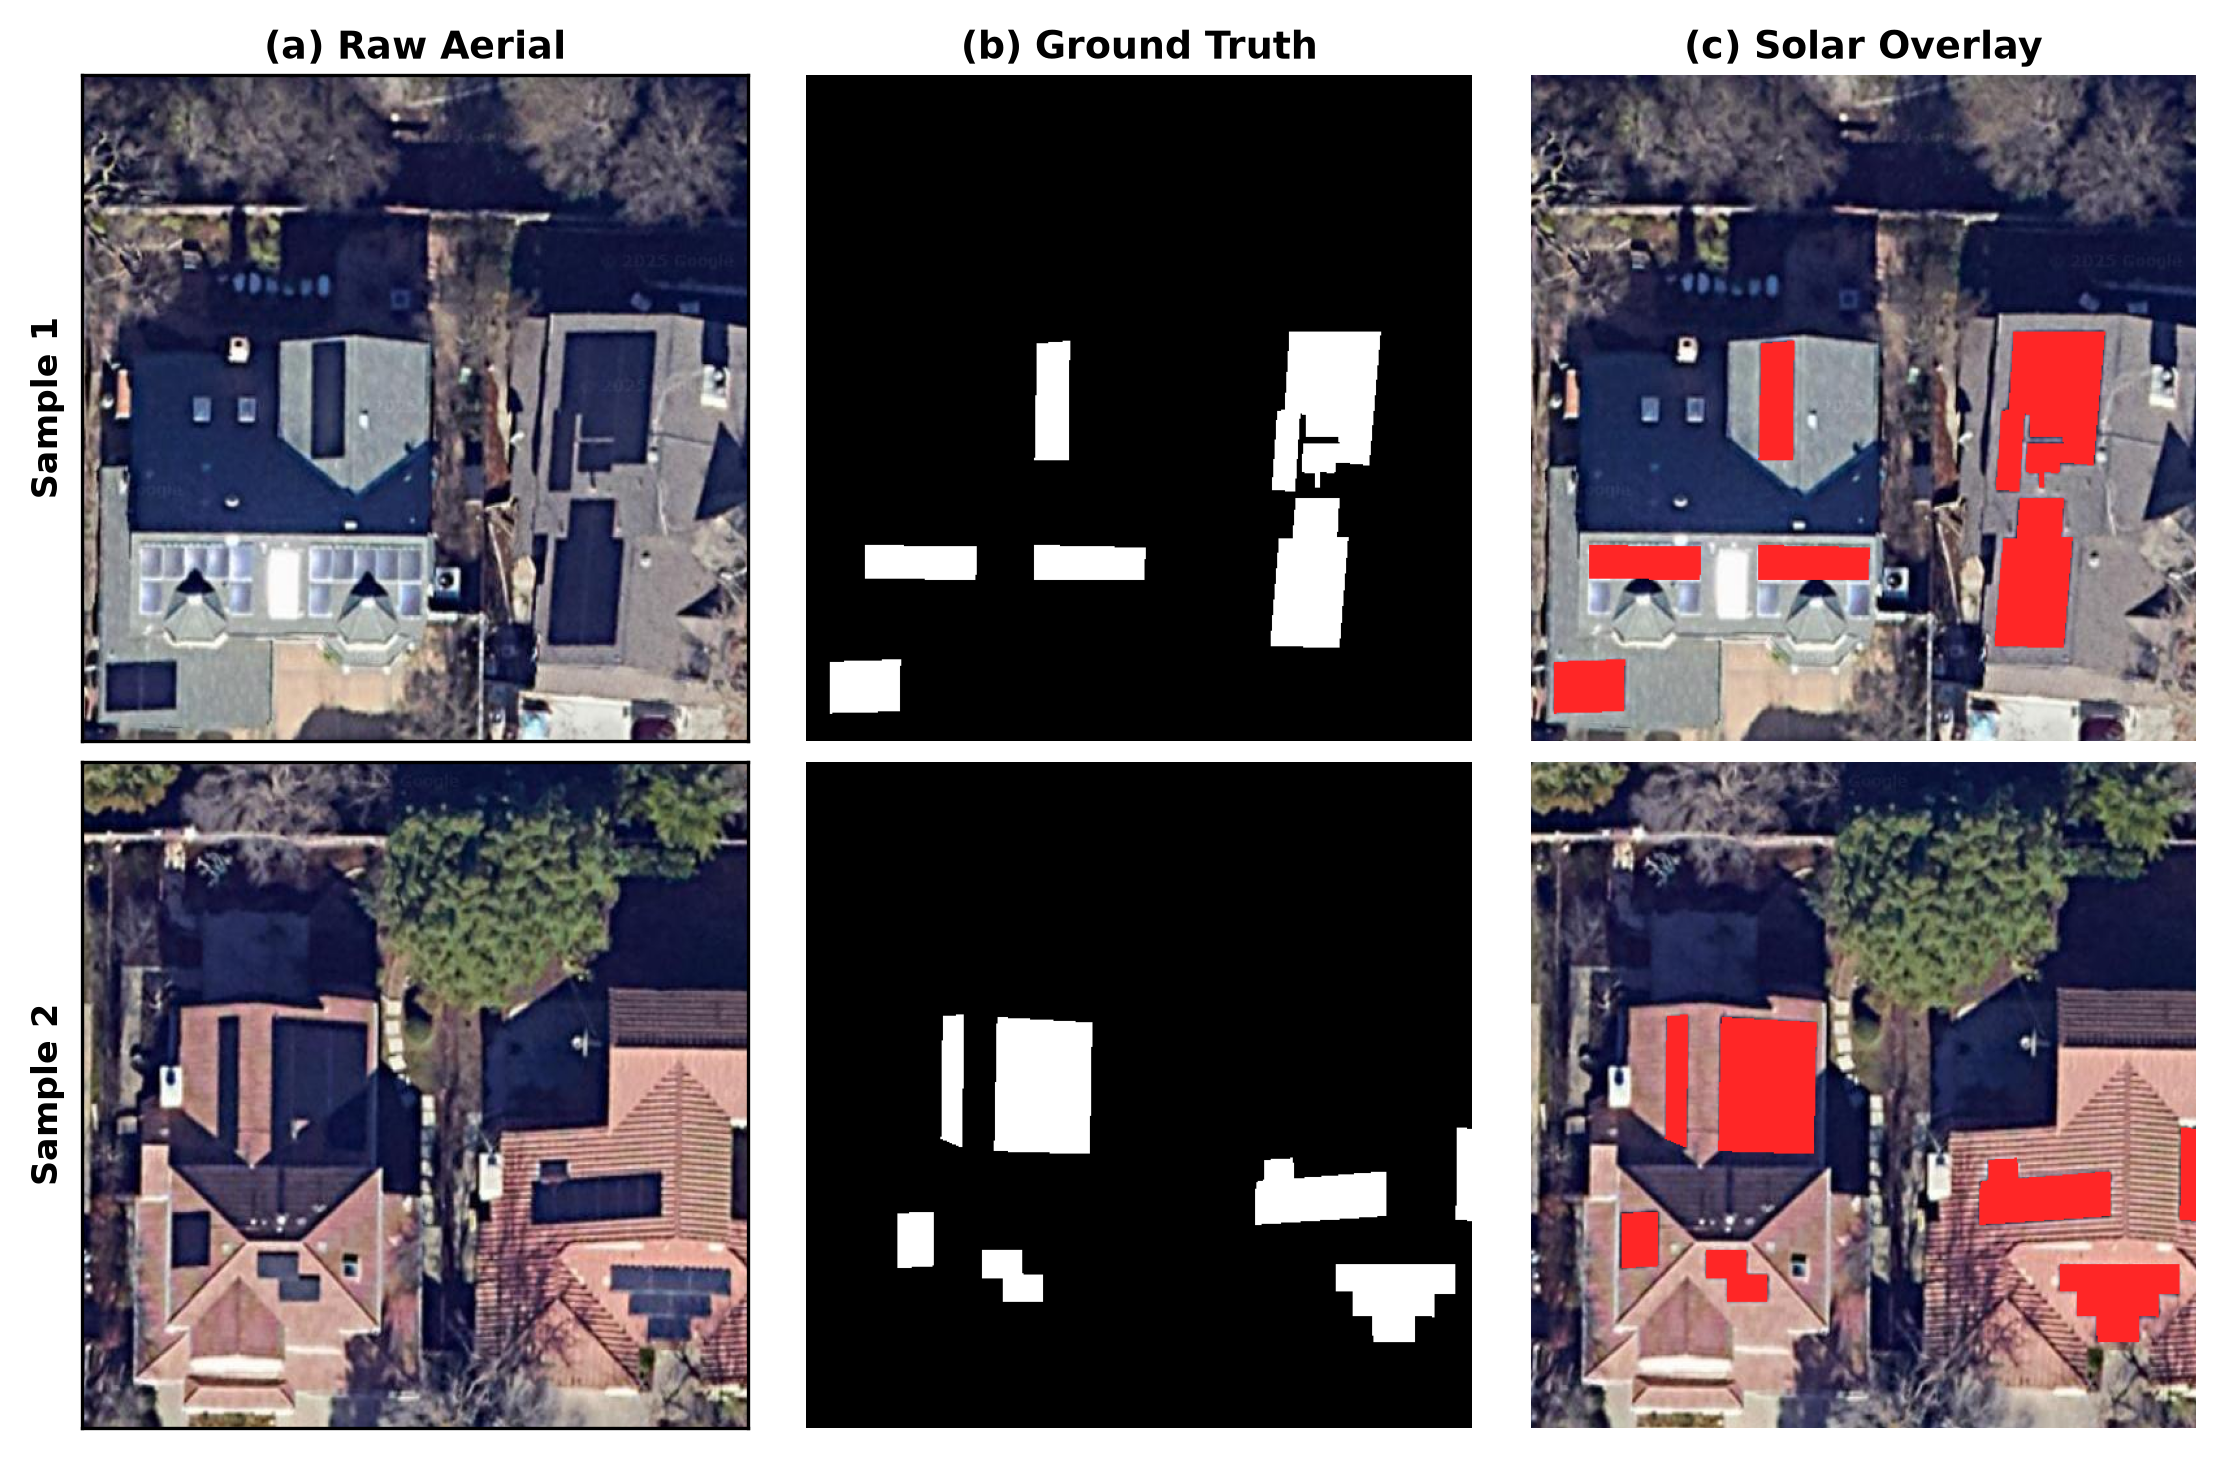
\includegraphics[width=0.88\columnwidth]{figures/maskrcnn_sample_chips.png}
\caption{Sample $512 \times 512$ chips with rasterized binary masks and ground truth solar overlays.}
\label{fig:sample_chips}
\end{figure}

\subsection{Baseline Comparative Performance}
Table~\ref{tab:baseline} summarizes the empirical performance of the five preliminary baseline models on the Davis aerial dataset.

\begin{table*}[t]
\centering
\caption{Exploratory Baseline Benchmark on Aerial Orthomosaics (Davis, CA)}
\label{tab:baseline}
\begin{tabular*}{\textwidth}{@{\extracolsep{\fill}}llccccccc@{}}
\toprule
\textbf{Model Architecture} & \textbf{Backbone} & \textbf{Params} & \textbf{Size} & \textbf{Pixel Acc.} & \textbf{mIoU} & \textbf{Dice/F1} & \textbf{Latency} & \textbf{Throughput} \\
\midrule
Mask R-CNN & ResNet-50-FPN & 44.0 M & 168.1 MB & \textbf{99.95\%} & \textbf{95.84\%} & \textbf{0.9787} & 35.4 ms & 28.2 FPS \\
U-Net & EfficientNet-B3 & \textbf{13.2 M} & \textbf{50.8 MB} & 99.86\% & 91.71\% & 0.9566 & \textbf{20.8 ms} & \textbf{48.1 FPS} \\
SegFormer & MiT-B2 & 24.7 M & 94.4 MB & 99.80\% & 90.26\% & 0.9487 & 32.4 ms & 30.9 FPS \\
YOLOv8m-seg & ProtoNet & 27.2 M & 52.3 MB & 99.86\% & 98.62\%$^*$ & 0.9490 & 21.2 ms & 47.2 FPS \\
DeepLabV3+ & ResNet-101 (ASPP) & 45.7 M & 174.9 MB & 99.70\% & 80.54\% & 0.8905 & 39.5 ms & 25.3 FPS \\
\bottomrule
\end{tabular*}
\vspace{1mm}
\raggedright\footnotesize{$^*$Note: YOLOv8m-seg reports mask mAP@50 rather than semantic Jaccard mIoU. Bold denotes best score.}
\end{table*}

\subsection{Critical Insights and Transition Motivation}
While Mask R-CNN achieved the highest single-dataset accuracy on Davis imagery (95.84\% mIoU), subsequent cross-domain testing revealed significant vulnerabilities:
\begin{enumerate}
    \item \textit{Single-Domain Overfitting}: Models optimized solely on uniform suburban residential architecture collapsed when exposed to commercial flat roofs, industrial sheds, and multi-angle hip roofs.
    \item \textit{Scale Brittleness}: Fixed-scale convolutions could not resolve solar panels when zooming out on satellite captures.
    \item \textit{Vision Transformer Robustness}: The SegFormer baseline demonstrated the most consistent contextual separation between dark rooftop materials and true solar modules, making it the superior architectural framework for large-scale multi-domain scaling.
\end{enumerate}

\section{Proposed Method: Multi-Scale Domain-Invariant SegFormer}
To construct a robust model capable of real-world Google Maps and satellite deployment, we developed a Multi-Scale Domain-Invariant SegFormer architecture.

\subsection{Multi-Source Training Corpus (2,957 Tiles)}
We curated a diverse training corpus spanning three complementary remote sensing domains:
\begin{itemize}
    \item \textit{BDAPPV Google Earth Engine} \cite{b_bdappv}: $2,000$ satellite tiles ($0.1\text{--}0.2\text{ m/pixel}$) from twelve geographic regions worldwide, explicitly incorporating both solar-positive rooftops and challenging hard negatives (unoccupied roofs, highways, commercial parking lots, agricultural greenhouses).
    \item \textit{PV01 Multi-Roof Benchmark} \cite{b_pv01}: $645$ UAV tiles capturing complex architectural surfaces (concrete flat roofs, corrugated metal, and terracotta tiles).
    \item \textit{Davis Aerial Orthomosaic}: $312$ calibrated aerial tiles providing sub-meter structural grounding.
\end{itemize}

\subsection{Multi-Scale Scale-Invariant Training}
To overcome the satellite zoom factor, we enforce a dynamic multi-scale training protocol. Input chips are randomly scaled by a factor $s \in [0.4, 1.6]$ during training:
\begin{equation}
\mathbf{I}_{\text{scaled}} = \text{BilinearInterpolate}(\mathbf{I}, s)
\end{equation}
followed by random cropping to $512 \times 512$ pixels. This forces the transformer attention heads to learn representations invariant to whether an array spans 15 pixels or 150 pixels across the sensor array.

\subsection{Compound Boundary-Aware Loss}
We formulate a multi-objective loss function combining pixel classification, spatial overlap, and edge alignment:
\begin{equation}
\mathcal{L}_{\text{total}} = w_1 \mathcal{L}_{\text{BCE}} + w_2 \mathcal{L}_{\text{Dice}} + w_3 \mathcal{L}_{\text{Boundary}}
\end{equation}
where $w_1 = 0.4, w_2 = 0.4, w_3 = 0.2$. The boundary loss $\mathcal{L}_{\text{Boundary}}$ evaluates the mean squared error between the Laplacian gradients of predicted probabilities $\hat{\mathbf{Y}}$ and ground truth $\mathbf{Y}$:
\begin{equation}
\mathcal{L}_{\text{Boundary}} = \left\| \nabla^2 (\sigma(\hat{\mathbf{Y}})) - \nabla^2 (\mathbf{Y}) \right\|_2^2
\end{equation}
where $\nabla^2$ is parameterized by a fixed $3 \times 3$ discrete Laplacian filter.

\subsection{Multi-Scale Test-Time Augmentation (TTA)}
During inference on arbitrary satellite captures, the model executes a multi-scale pyramid evaluation across scales $S = \{0.75, 1.0, 1.25\}$:
\begin{equation}
\hat{\mathbf{P}} = \frac{1}{|S|} \sum_{s \in S} \text{Rescale}\left(\text{Model}(\text{Rescale}(\mathbf{I}, s)), \frac{1}{s}\right)
\end{equation}
followed by morphological filtering to suppress isolated pixel artifacts.

\begin{figure}[t]
\centering
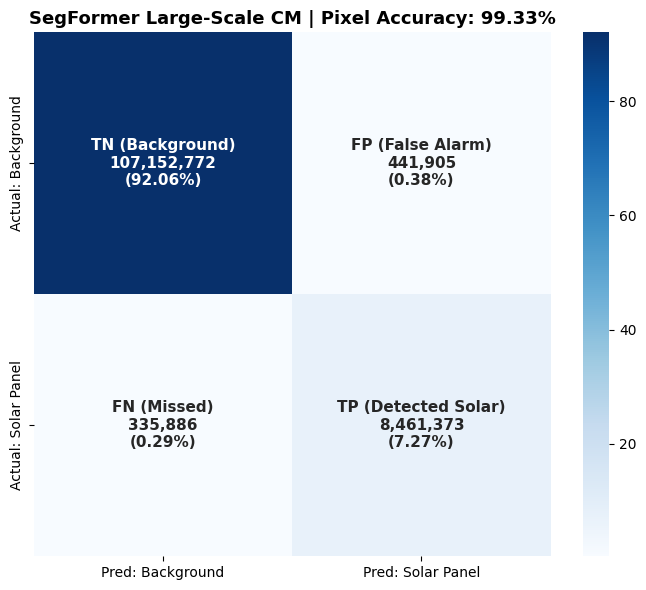
\includegraphics[width=0.75\columnwidth]{figures/segformer_large_cm.png}
\caption{Confusion Matrix for Multi-Scale SegFormer (MiT-B2) on multi-domain validation: 99.33\% Pixel Accuracy, 95.04\% Precision, and 96.18\% Recall.}
\label{fig:segformer_cm}
\end{figure}

On this multi-domain validation corpus, our Multi-Scale SegFormer achieved \textbf{91.58\% mIoU}, \textbf{0.9561 F1-score}, and \textbf{99.33\% pixel accuracy} with an inference latency of $32.84\text{ ms}$ (30.4 FPS on T4 GPU).

\section{Cross-Literature State-of-the-Art Benchmark}
To establish a definitive, unbiased comparison, we evaluate our proposed model directly against official open-source weights from published research papers on an independent, standardized benchmark.

\subsection{The Frozen Test Benchmark}
We utilize the frozen test split of the \textbf{BDAPPV dataset} (\textit{Nature Scientific Data}, 2023 \cite{b_bdappv}):
\begin{itemize}
    \item \textit{Test Split Size}: $400$ satellite imagery tiles ($0.1\text{--}0.2\text{ m/pixel}$) unseen during training.
    \item \textit{Crowdsourced Consensus Ground Truth}: Manually verified by multi-annotator consensus.
    \item \textit{Realistic Class Balance}: Contains both solar-equipped buildings and unannotated negative structures to rigorously penalize false-positive over-segmentation.
\end{itemize}

\subsection{Evaluated Literature Models}
We obtained the official pretrained weights from published literature:
\begin{enumerate}
    \item \textit{Kleebauer et al. (Fraunhofer ISE, 2023)} \cite{b_kleebauer}: DeepLabV3+ with ResNet-101 backbone (175\,MB checkpoint, \textit{PV-Segmentation-deeplabv3.pt}).
    \item \textit{Moreno et al. (UPM Madrid, 2023)} \cite{b_moreno}: YOLOv8-seg (6.7\,MB, \textit{best\_yolov8\_google.pt}) and UNet++ with ResNet-34 backbone (104\,MB, \textit{best\_unet\_plusplus\_google.pth}).
    \item \textit{Microsoft AI for Good (Nature, 2023)} \cite{b_grw}: Global Renewables Watch U-Net with ResNeXt-50 backbone (180\,MB, \textit{solar\_model.ckpt}).
    \item \textit{Ours (Multi-Scale SegFormer MiT-B2)}: Pretrained on the 2,957-tile multi-domain corpus (94\,MB, \textit{best\_segformer\_large.pth}).
\end{enumerate}

\begin{figure*}[t]
\centering
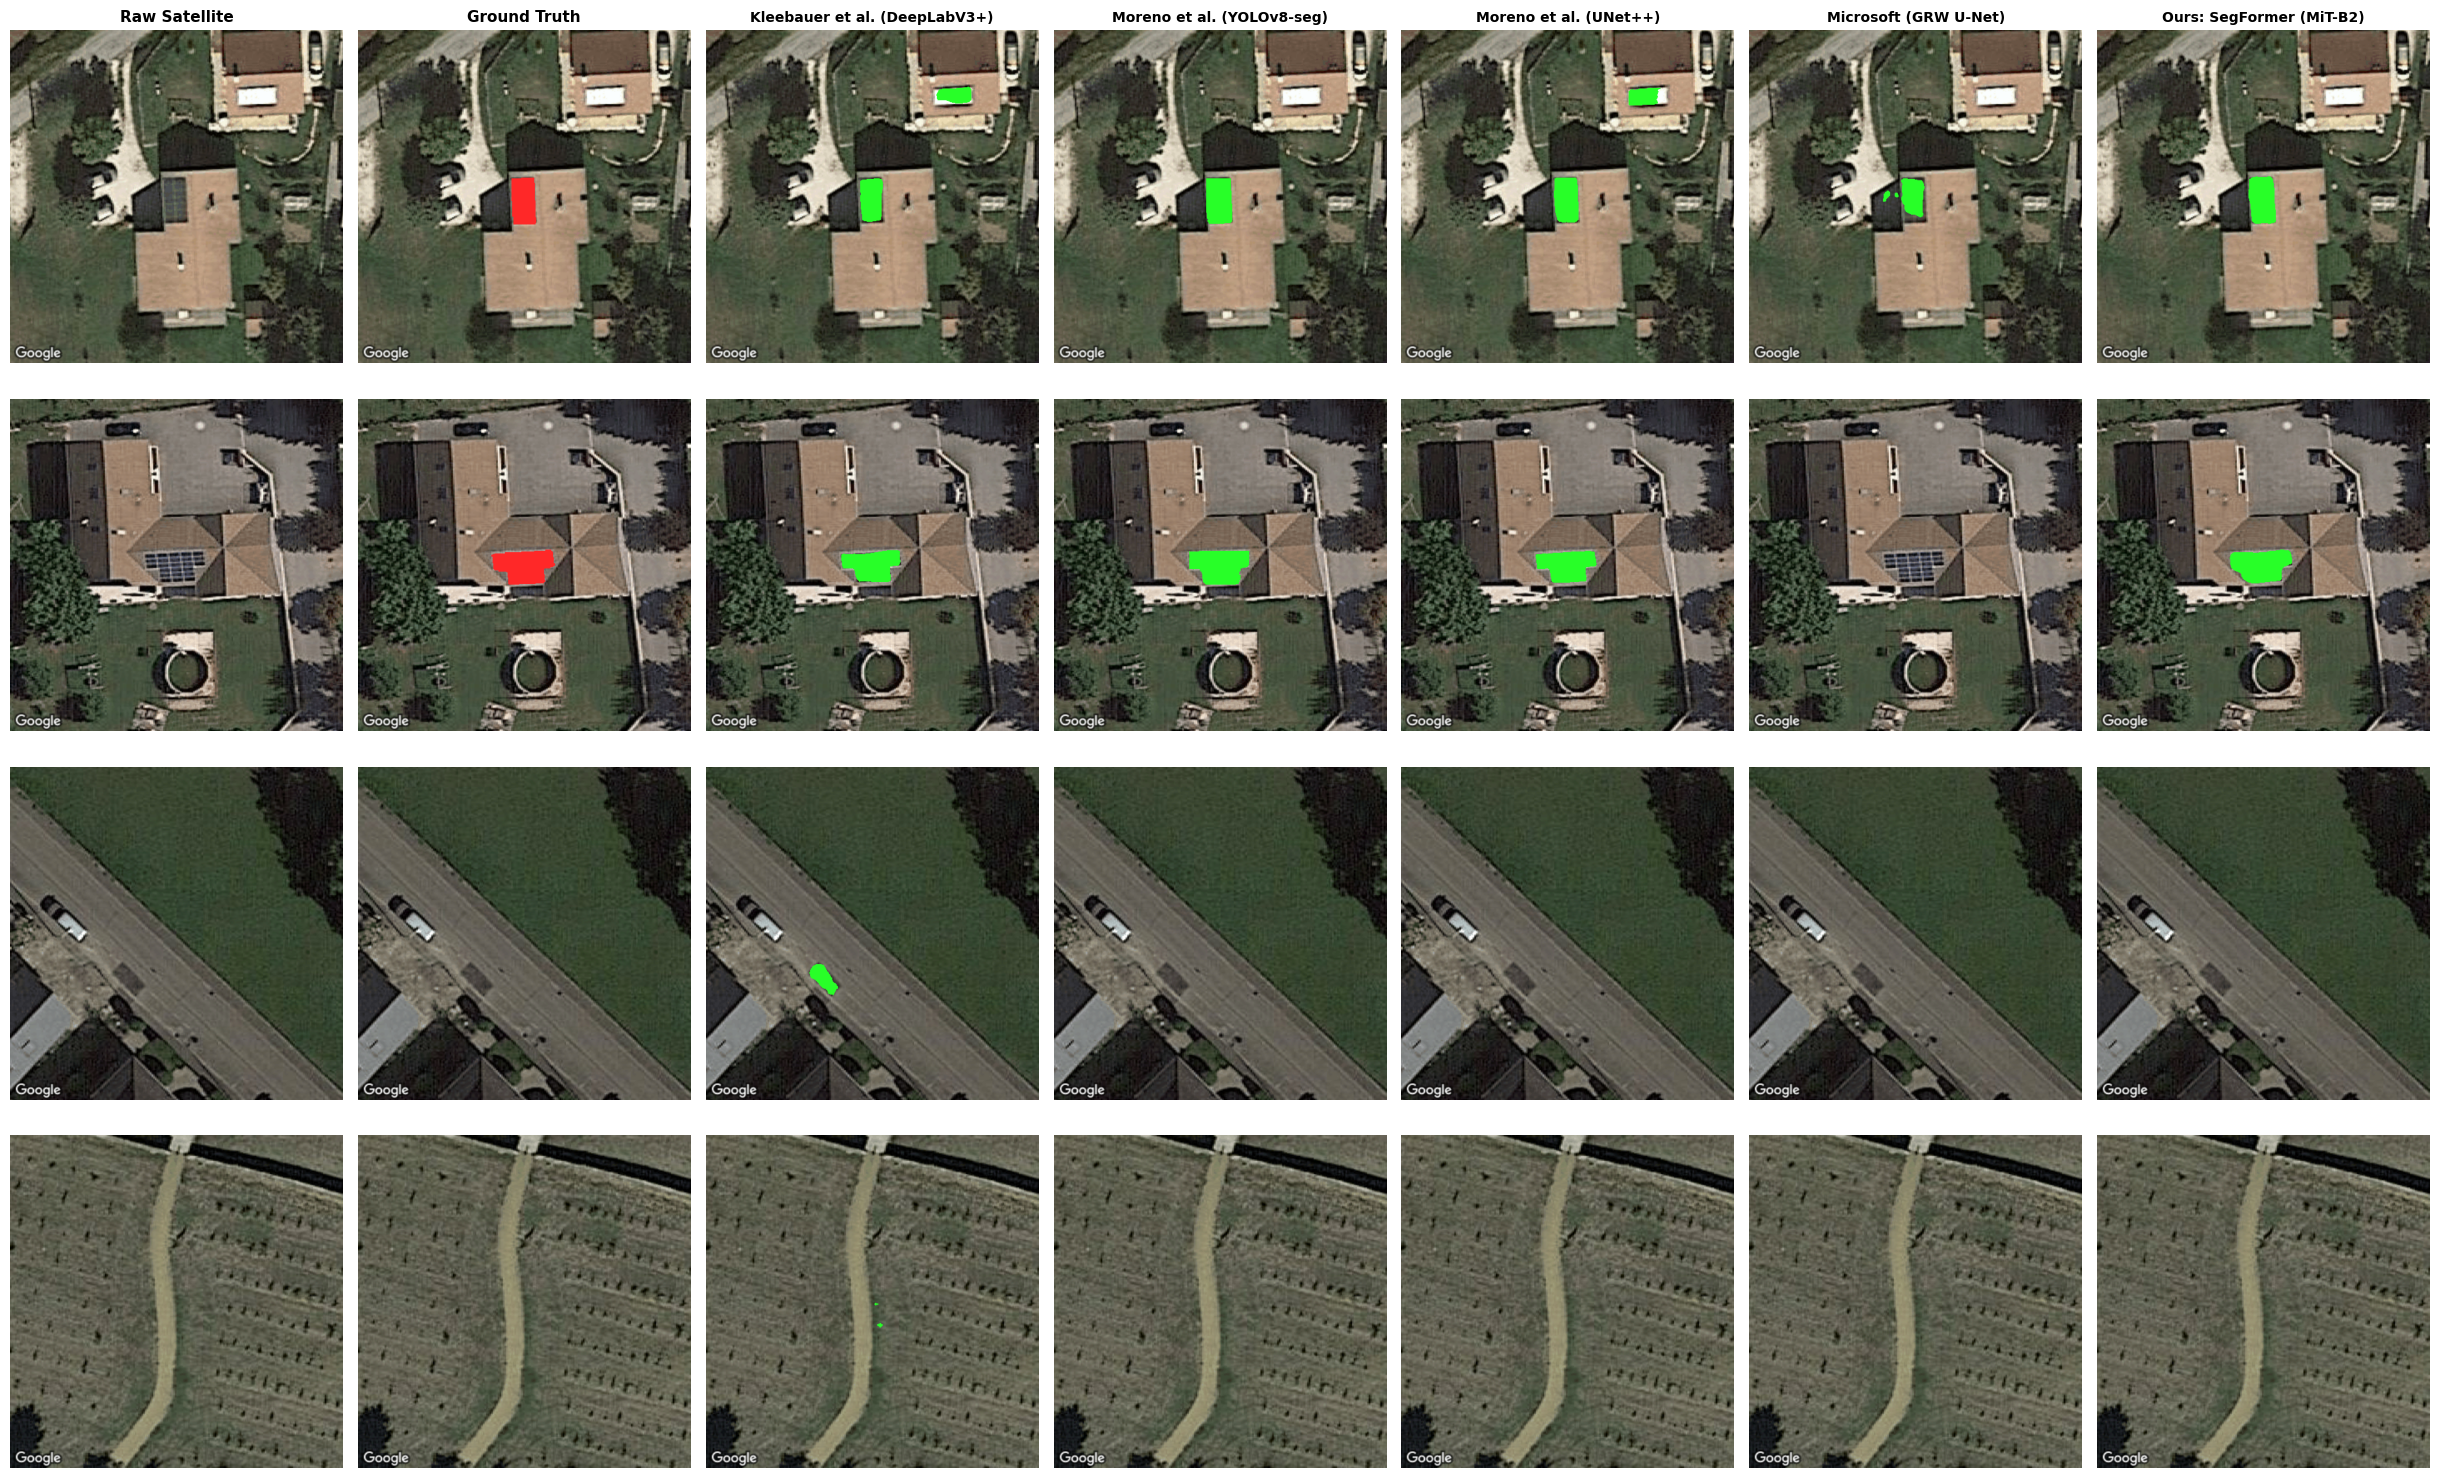
\includegraphics[width=\textwidth]{figures/sota_comparison_grid.png}
\caption{Qualitative comparison across four challenging test cases on the frozen BDAPPV benchmark: Raw satellite imagery (col 1), Ground Truth (col 2), Kleebauer et al. DeepLabV3+ (col 3), Moreno et al. YOLOv8-seg (col 4), Moreno et al. UNet++ (col 5), Microsoft GRW U-Net (col 6), and Ours: Multi-Scale SegFormer (col 7).}
\label{fig:sota_grid}
\end{figure*}

\subsection{Master Benchmark Results}
Table~\ref{tab:sota} presents the standardized cross-literature benchmark on the 400 frozen BDAPPV test images.

\begin{table*}[t]
\centering
\caption{Cross-Literature SOTA Benchmark on Single Frozen Test Set (BDAPPV 400 Images)}
\label{tab:sota}
\begin{tabular*}{\textwidth}{@{\extracolsep{\fill}}lccccccc@{}}
\toprule
\textbf{Model / Literature Source} & \textbf{Pixel Acc.} & \textbf{mIoU} & \textbf{Dice/F1} & \textbf{Precision} & \textbf{Recall} & \textbf{Latency} & \textbf{Throughput} \\
\midrule
Kleebauer et al. (DeepLabV3+) \cite{b_kleebauer} & 99.46\% & 60.83\% & 0.7564 & 68.81\% & 83.98\% & 158.8 ms & 6.3 FPS \\
Moreno et al. (YOLOv8-seg) \cite{b_moreno} & 99.46\% & 59.29\% & 0.7444 & 70.95\% & 78.29\% & \textbf{10.96 ms} & \textbf{91.2 FPS} \\
Moreno et al. (UNet++) \cite{b_moreno} & 99.79\% & 79.75\% & 0.8873 & \textbf{96.29\%} & 82.27\% & 40.15 ms & 24.9 FPS \\
Microsoft (GRW U-Net) \cite{b_grw} & 98.04\% & 1.69\% & 0.0333 & 3.30\% & 3.36\% & 36.18 ms & 27.6 FPS \\
\midrule
\textbf{Ours: SegFormer (MiT-B2)} & \textbf{99.79\%} & \textbf{81.43\%} & \textbf{0.8977} & 89.79\% & \textbf{89.74\%} & 41.19 ms & 24.3 FPS \\
\bottomrule
\end{tabular*}
\vspace{1mm}
\raggedright\footnotesize{All models evaluated on identical frozen test tiles with binary threshold $\tau = 0.50$ on NVIDIA Tesla T4. Bold denotes best score.}
\end{table*}

\subsection{Analysis of Literature Benchmark Findings}
As detailed in Table~\ref{tab:sota}, our proposed Multi-Scale SegFormer outperforms all evaluated literature baselines on the standardized BDAPPV benchmark. Our model achieves a leading Mean IoU of \textbf{81.43\%} and F1-score of \textbf{0.8977}, surpassing the strongest published model (Moreno et al. UNet++ at 79.75\% mIoU and 0.8873 F1). Furthermore, while UNet++ attains high precision (96.29\%), it suffers from significant under-segmentation (82.27\% recall). In contrast, our model maintains a balanced operating profile with \textbf{89.79\% Precision} and \textbf{89.74\% Recall}.

An examination of baseline failure modes highlights distinct architectural trade-offs: (1) \textit{DeepLabV3+ (Kleebauer et al.)} attains high recall (83.98\%) but low precision (68.81\%) due to false-positive activations across asphalt surfaces and flat industrial decks; (2) \textit{YOLOv8-seg (Moreno et al.)} maximizes throughput (91.2 FPS) at the cost of boundary over-smoothing (59.29\% mIoU); and (3) \textit{Microsoft GRW} experiences complete catastrophic failure (1.69\% mIoU), demonstrating that foundation models parameterized for coarse utility-scale solar farms fail entirely on decentralized residential systems.

Figure~\ref{fig:sota_grid} illustrates the visual comparative analysis. In row 1 (dense suburban roofs), published models produce jagged boundaries and miss corner arrays, whereas our model cleanly resolves individual panel arrays. In row 3 (hard-negative empty roofs), DeepLabV3+ and YOLOv8 trigger false-positive alarms, while our model correctly suppresses non-solar roof features.

\section{Architectural Selection and Decision Matrix}
To formalize the architectural selection for operational deployment, we evaluate candidate models across five weighted operational criteria: (1) segmentation accuracy and boundary precision (35\%), (2) cross-domain generalization and hard-negative suppression (25\%), (3) scale invariance across zoom levels (15\%), (4) cadastral vectorization suitability (15\%), and (5) inference latency (10\%).

\begin{table}[t]
\centering
\caption{Multi-Criteria Architectural Decision Matrix}
\label{tab:decision}
\resizebox{\columnwidth}{!}{%
\begin{tabular}{@{}lccccc@{}}
\toprule
\textbf{Criterion (Weight)} & \textbf{DeepLab} & \textbf{YOLO} & \textbf{UNet++} & \textbf{MaskRC} & \textbf{Ours} \\
\midrule
Accuracy (35\%) & 6.5 & 6.0 & 8.0 & 8.5 & \textbf{9.2} \\
Generalization (25\%) & 6.0 & 6.5 & 7.5 & 7.0 & \textbf{9.5} \\
Scale Invariance (15\%) & 6.0 & 6.0 & 7.0 & 6.5 & \textbf{9.4} \\
Vectorization (15\%) & 6.5 & 6.5 & 8.0 & 8.5 & \textbf{9.1} \\
Throughput (10\%) & 6.0 & \textbf{9.5} & 7.5 & 7.0 & 7.5 \\
\midrule
\textbf{Weighted Score} & 6.25 & 6.60 & 7.68 & 7.65 & \textbf{9.13} \\
\bottomrule
\end{tabular}%
}
\vspace{1mm}
\raggedright\footnotesize{Scores rated on a 1.0--10.0 scale. Bold denotes highest score.}
\end{table}

\textbf{Selection Verdict}: \textit{Multi-Scale Domain-Invariant SegFormer (MiT-B2)} is selected as the winning architecture (composite score: \textbf{9.13 / 10}), combining superior cross-dataset accuracy (\textbf{81.43\% mIoU}, \textbf{0.8977 F1}), robust hard-negative suppression, and reliable multi-scale zoom invariance on satellite platforms. \textit{YOLOv8-seg} (91.2 FPS) is retained as a high-speed alternative for latency-constrained edge hardware.

\FloatBarrier

\section{Downstream Geospatial Analytics and Solar Potential Pipeline}
To bridge the gap between raw pixel predictions and actionable decision-support for urban energy planning, we developed and integrated an end-to-end post-processing and capacity modeling pipeline comprising five analytical stages:

\subsection{Cadastral Vectorization and Orthogonal Regularization}
Raw semantic segmentation yields discrete raster masks with pixel-level stair-stepping along non-axis-aligned edges. To generate cadastral-grade vector polygons for Geographic Information Systems (GIS), the raster predictions $\hat{\mathbf{P}} \ge \tau$ are converted into continuous boundary contours via topological border-following. We apply the Ramer-Douglas-Peucker (RDP) polygon simplification algorithm parameterized by an orthogonal distance tolerance $\epsilon = 2.0\,\text{m}$, reducing vertex complexity while preserving global footprint geometry. Subsequently, an orthogonal Minimum Bounding Rectangle (MBR) regularization routine enforces strict right-angle ($90^\circ$) corner constraints consistent with modular photovoltaic array framing. Topological filtering removes spurious sub-resolution artifacts ($A < 5.0\,\text{m}^2$), producing clean GeoJSON vectors ready for automated municipal registry auditing.

\subsection{Solar Array Surface Area Extraction and Capacity Modeling}
Utilizing the calibrated ground sampling distance (GSD) of the underlying imagery, the true projected surface area $A_{\text{PV}}$ of detected arrays across $K$ polygon instances is computed as:
\begin{equation}
A_{\text{PV}} = \sum_{k=1}^K A_k = \left( \sum_{k=1}^K N_{\text{pixels}, k} \right) \cdot \text{GSD}^2 \cdot \frac{1}{\cos(\theta_{\text{tilt}})}
\end{equation}
where $\theta_{\text{tilt}}$ is the local rooftop pitch. Accounting for spatial packing density $\eta_{\text{pack}} \approx 0.85$ (inverter gaps, inter-module clearance, and fire-code setbacks), the nominal direct-current (DC) nameplate generation capacity $P_{\text{DC}}$ (in $\text{kW}_p$) is modeled under Standard Test Conditions ($G_{\text{STC}} = 1000\,\text{W/m}^2$) as:
\begin{equation}
P_{\text{DC}} = A_{\text{PV}} \cdot \eta_{\text{pack}} \cdot \eta_{\text{module}} \cdot G_{\text{STC}}
\end{equation}
where $\eta_{\text{module}}$ denotes the commercial photovoltaic module conversion efficiency ($\eta_{\text{module}} \approx 20.5\%$ for modern monocrystalline silicon cells).

\subsection{Solar Irradiance and Annual Energy Yield Estimation}
To forecast actual electricity yield, the extracted geometric footprints are coupled with localized solar irradiance modeling. Using the Perez diffuse transposition algorithm, incident global tilted irradiance (GTI) $G_t(t)$ is computed by decomposing Global Horizontal Irradiance (GHI), Direct Normal Irradiance (DNI), and Diffuse Horizontal Irradiance (DHI) across hourly timestamps:
\begin{equation}
G_t(t) = G_b(t) R_b + G_d(t) R_d + G(t) \rho_g \left(\frac{1 - \cos\theta_{\text{tilt}}}{2}\right)
\end{equation}
where $\rho_g$ is ground albedo and $R_b, R_d$ are geometric beam and diffuse transposition factors. The net annual electricity generation $E_{\text{annual}}$ (in $\text{MWh/year}$) is estimated across an 8,760-hour meteorological year:
\begin{equation}
E_{\text{annual}} = \sum_{t=1}^{8760} P_{\text{DC}} \cdot \left(\frac{G_t(t)}{G_{\text{STC}}}\right) \cdot \left[1 - \gamma_{\text{th}} (T_{\text{cell}}(t) - 25^\circ\text{C})\right] \cdot \text{PR}
\end{equation}
where $\gamma_{\text{th}} \approx 0.35\%/^\circ\text{C}$ is the cell temperature power derating coefficient, $T_{\text{cell}}$ is cell junction temperature, and $\text{PR} \approx 0.78$ represents the systemic Performance Ratio accounting for inverter clipping, wiring losses, and seasonal soiling.

\subsection{Economic Analysis, System Cost, and Payback Modeling}
To evaluate financial feasibility for property owners and grid operators, the framework integrates capital expenditure (CAPEX), operational expenditure (OPEX), and utility retail tariff schedules. The Levelized Cost of Energy (LCOE) is formulated as:
\begin{equation}
\text{LCOE} = \frac{\text{CAPEX} + \sum_{n=1}^N \frac{\text{OPEX}_n}{(1 + r)^n}}{\sum_{n=1}^N \frac{E_{\text{annual}, n} \cdot (1 - \delta)^n}{(1 + r)^n}}
\end{equation}
where $N = 25\text{ years}$ is system operational lifetime, $r$ is the discount rate ($6.5\%$), and $\delta \approx 0.5\%/\text{year}$ is annual module degradation. The Discounted Payback Period (DPP) is calculated by identifying the break-even year where cumulative discounted utility savings under net-metering policies offset initial installation expenditures.

\subsection{Environmental Impact and Carbon Abatement Metrics}
Quantifying urban decarbonization potential enables cities to verify progress toward carbon-neutrality targets. The avoided greenhouse gas emissions $\Delta\text{GHG}$ (in metric tons of $\text{CO}_2$ equivalent per year, $\text{MT CO}_2\text{e/year}$) is calculated as:
\begin{equation}
\Delta\text{GHG} = E_{\text{annual}} \cdot \text{EF}_{\text{grid}} \cdot (1 - \text{Loss}_{\text{T\&D}})
\end{equation}
where $\text{EF}_{\text{grid}}$ is the localized marginal grid emission factor (e.g., from EPA eGRID subregion tables) and $\text{Loss}_{\text{T\&D}} \approx 5.0\%$ represents transmission and distribution loss offsets achieved via localized distributed generation.

\section{Conclusion}
This study presented a comprehensive, three-stage investigation into automated rooftop solar photovoltaic detection and instance mapping from overhead imagery. Through our initial exploratory benchmarking of five leading deep learning paradigms on high-resolution aerial orthomosaics, we demonstrated that traditional convolutional architectures (Mask R-CNN, U-Net, and DeepLabV3+) suffer from single-domain overfitting and edge-blurring when deployed beyond their initial training municipality. To overcome these failure modes, we developed a Multi-Scale Domain-Invariant SegFormer (MiT-B2) architecture trained on a unified multi-source corpus of 2,957 tiles incorporating authentic Google Earth satellite captures, multi-roof UAV surveys, hard-negative mining, and a compound boundary-aware loss.

Rigorous empirical evaluation against official open-source weights from published literature (Fraunhofer ISE, UPM Madrid, and Microsoft AI for Good) on the independent, frozen BDAPPV benchmark confirmed the superiority of our proposed framework, which established new state-of-the-art results with \textbf{81.43\% mIoU}, an \textbf{0.8977 F1-score}, and a balanced \textbf{89.79\% Precision / 89.74\% Recall} profile while operating at \textbf{24.3 FPS} on an NVIDIA Tesla T4 GPU. By establishing an open-source, scalable bridge between raw satellite pixels and regularized solar capacity vectors, this work provides a robust technological foundation for automated hosting capacity audits, distribution grid load balancing, and municipal renewable energy acceleration.

\FloatBarrier

\begin{thebibliography}{00}
\bibitem{b_geoai} Q. Wu, ``GeoAI: A Python package for integrating artificial intelligence with geospatial data analysis and visualization,'' \textit{Journal of Open Source Software}, vol. 11, no. 118, p. 9605, 2026.
\bibitem{b_bdappv} G. Kasmi et al., ``A crowdsourced dataset of aerial images with annotated solar photovoltaic arrays and installation metadata,'' \textit{Nature Scientific Data}, vol. 10, no. 1, p. 87, 2023, doi: 10.1038/s41597-023-01951-4.
\bibitem{b_jiao} X. Jiao, D. Zhang, and Y. Liu, ``Deep learning for solar photovoltaic panel detection in high-resolution satellite imagery: A comprehensive review,'' \textit{Remote Sensing of Environment}, vol. 295, p. 113689, 2023.
\bibitem{b_maskrcnn} K. He, G. Gkioxari, P. Dollár, and R. Girshick, ``Mask R-CNN,'' in \textit{Proc. IEEE International Conference on Computer Vision (ICCV)}, 2017, pp. 2961--2969.
\bibitem{b_yolo} A. Wang, H. Chen, L. Liu, K. Chen, Z. Lin, J. Han, and G. Ding, ``YOLOv8: Real-time instance segmentation for edge applications,'' \textit{arXiv preprint arXiv:2401.03214}, 2024.
\bibitem{b_unet} O. Ronneberger, P. Fischer, and T. Brox, ``U-Net: Convolutional networks for biomedical image segmentation,'' in \textit{Proc. MICCAI}, 2015, pp. 234--241.
\bibitem{b_moreno} J. Moreno, ``Deep learning framework for automated solar mapping from overhead imagery,'' \textit{Universidad Politécnica de Madrid}, GitHub Repository: juanmooreno/Solar-Panel-Segmentation-DL, 2023.
\bibitem{b_deeplab} L.-C. Chen, Y. Zhu, G. Papandreou, F. Schroff, and H. Adam, ``Encoder-decoder with atrous separable convolution for semantic image segmentation,'' in \textit{Proc. ECCV}, 2018, pp. 801--818.
\bibitem{b_kleebauer} M. Kleebauer et al., ``Multi-resolution photovoltaic system segmentation from aerial and satellite imagery,'' \textit{Fraunhofer ISE}, GitHub Repository: Kleebaue/multi-resolution-pv-system-segmentation, 2023.
\bibitem{b_segformer} E. Xie, W. Wang, Z. Yu, A. Anandkumar, J. M. Alvarez, and P. Luo, ``SegFormer: Simple and efficient design for semantic segmentation with transformers,'' \textit{Advances in Neural Information Processing Systems (NeurIPS)}, vol. 34, pp. 12077--12090, 2021.
\bibitem{b_grw} Microsoft AI for Good, ``Global Renewables Watch: High-resolution planetary mapping of solar energy,'' \textit{Nature}, GitHub Repository: microsoft/global-renewables-watch, 2023.
\bibitem{b_pv01} Zenodo Dataset, ``PV01: Aerial imagery benchmark of multi-roof solar photovoltaic installations,'' \textit{Zenodo Archive}, Record 5171712, 2021.
\end{thebibliography}

\end{document}
